\section{Overview of the Proposed Research and Our Preliminary Result}
\label{sec:overview}

\begin{figure}[!t]
  \centering
  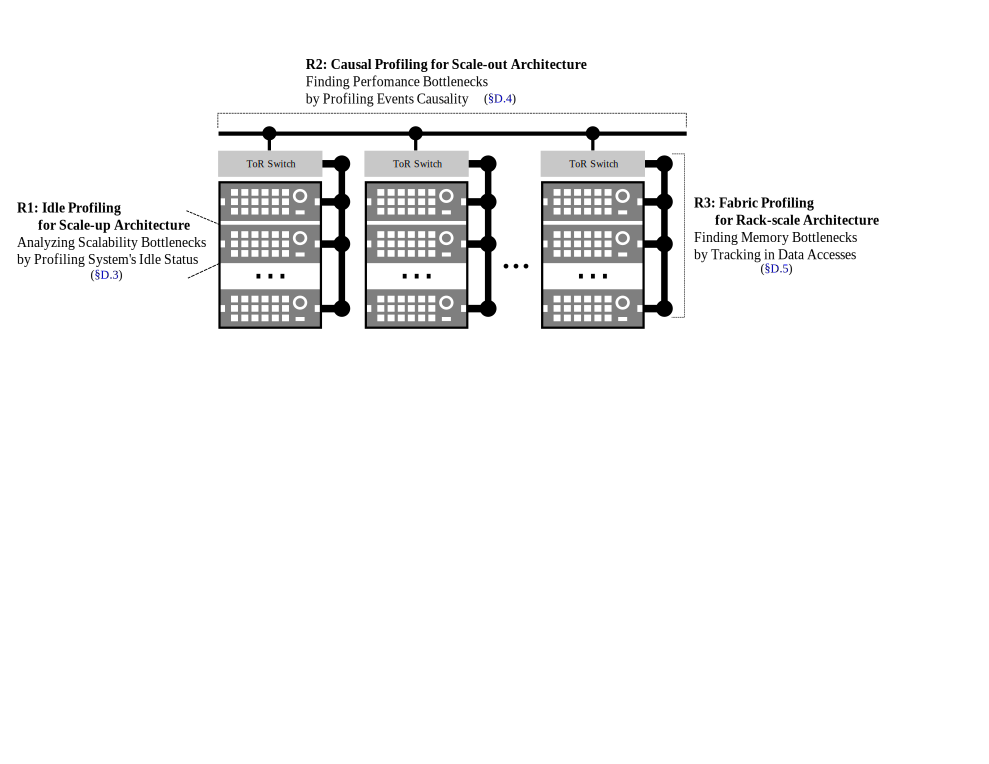
\includegraphics[width=0.99\textwidth]{fig/proj-overview}
  \caption{How each research thrust is positioned to find scalability
    bottlenecks in the extreme scale parallelism. The proposed
    research aims to develop techniques and tools to find scalability
    bottlenecks in three different scaling architectures: scale-up,
    scale-out, and rack-scale architectures. In R1, we will
    develop techniques and tools, named {\em idle profiling}, to
    analyze scalability bottlenecks in scale-up systems by analyzing
    a system's idle status. In R2, we will develop techniques and
    tools, named {\em causal profiling}, to find performance
    bottlenecks that affect the end-to-end performance in
    scale-out architectures. In R3, we will develop techniques
    and tools, named {\em fabric profiling}, to find memory hotspots
    and latency spikes caused by the hotspots in rack-scale
    architectures connected via a fabric network (e.g.,
    InfiniBand, Omni-Path).}
  \label{f:overview}
  \vspace{-5px}
\end{figure}

The proposed research has three main goals:
(1) analyzing scalability bottlenecks in a scale-up system by
profiling the idle state of a system;
(2) finding performance bottlenecks in a scale-out system by
profiling the event causality;
and (3) identifying memory bottlenecks in a rack-scale system by profiling
data accesses.

These three research thrust complement  each other, as
illustrated in~\autoref{f:overview}.
%
To find scalability bottlenecks in a scale-up system, we will profile which
CPUs are idle or why CPU cycles are wasted while spinning (i.e., idle state).
As a result of profiling, we will analyze which tasks are waiting for what and
how critical sections are related to each other.
We will then present dependencies of tasks and critical sections as a weighted
graph, named an idle graph, that will provide a holistic view on scalability
bottlenecks in a system including OS kernel and libraries.
In addition, we will also suggest some of the best optimization candidates among
the critical sections by virtually speeding up each critical sections.
We will develop several novel techniques (e.g., finding spin loops
in binary files, dynamic profiling with minimal profiling overhead, etc). We
present the preliminary design of the idle profiler in~\autoref{sec:idleprofile}.

To determine how much the end-to-end performance will be affected by
optimizing a sub-task of a distributed application,
we will develop causal profiling techniques,
which suggest critical performance bottlenecks as some of the best
optimization candidates. To deal with the complexity of distributed
systems, we will take an empirical approach by extending the virtual
speedup techniques for distributed systems,
named distributed virtual speedup. Instead of actually
speeding up a sub-task, we will virtually speed up a sub-task by
slowing all the others to see its impact on end-to-end
performance. To transparently profile a distributed application
without any modification, we will tap on the RPC layer of a
distributed framework. While such an empirical approach will be accurate,
the time and cost to get the best plausible candidates will be
prohibitively high because of its huge search space (e.g., the number of
sub-tasks \x the number of running nodes). To effectively prune the
search space, we plan to explore stochastic techniques, which exploit
the execution structure of a distributed application. We present
details of our proposed research in~\autoref{sec:causalprofile}.

To identify memory bottlenecks and latency spikes in a fabric network,
which has extremely low access latency, we will take
a hardware/software co-profiling approach. We will develop
a performance monitoring unit (PMU) that profiles memory access frequency
and latency using an FPGA in a NIC. Even using our performance
monitoring unit, profiling overhead and the size of profiled data will
be prohibitively huge if we monitor every memory access. Thus, we plan
to take a hierarchical approach:
we first profile the frequency of the memory access using the NIC PMU;
for the frequently accessed memory addresses, we will profile their
access latency using the PMU and collect the latency of selected
frequently accessed memory locations in a fabric network;
for high-latency memory addresses, we will profile code paths
accessing those addresses using software profiling techniques. We
provide our research plan on this area in~\autoref{sec:fabricprofile}.

\paragraph{Related Projects Led by PIs}
% unique roles by each
Both PIs bring unique perspectives and expertise to make
this project successful.
%
In the past, PI Min worked in industry for more than 10 years
as a principal software engineer
who had led the design and engineering
of the Linux-based mobile platform (Tizen), Java virtual machine (J9),
and high-performance server products (WebSphere),
in Samsung Electronics and IBM.
%
Since joining academia, he has been working on designing a new
parallel runtime for a scale-up
machine~\cite{Min:DANBI:PACT13} and concurrent data structures, such
as the FIFO queue~\cite{Min:LECDQ:TPDS15}, bringing solid experience in
software designed for scale-up architectures.
%
PI Kim has been working on the recovery of
distributed applications~\cite{chandra:aire},
distributed storage systems on top of commodity cloud
services~\cite{han:metasync, han:metasync2},
and hardware-assisted data-flow isolation using FPGA~\cite{song:hdfi}.
%
As a lead PI of the DARPA Extreme DDoS Defense (XD3)
project~\cite{xd3:web}, he has been working on high-performance
FPGA-attached NIC devices and Internet-scale services.

% about recent collaboration
Both PI Min and PI Kim have recently started collaborating on
building scalable operating systems on a scale-up architecture.
%
Two notable works include
a scalable synchronization primitive,
called OTicket~\cite{kashyap:oticket, kashyap:oppspinlocks},
and a scalability benchmark for file systems, called
FxMark~\cite{min:fxmark}.
%
OTicket solves the lock holder preemption problem
in a virtualized environment
by opportunistically spinning more on the contending spinlocks
based on their waiting orders.
%
FxMark~\cite{min:fxmark} provides a way
to emphatically identify scalability bottlenecks
of Linux file system implementations.
It systematically stresses (i.e., 19 micro-benchmarks)
each component of Linux file systems 
to highlight the scalability behaviors
(e.g., it found 25 scalability bottlenecks in popular Linux file
systems such as ext4 and btrfs).
%
The outcomes of these two projects are remarkable.
%
The new spinlock design proposed by OTicket
was recently adopted by the mainline Linux kernel~\cite{waiman:spinlock},
and the FxMark benchmark was recently adopted
by the SUSE's QoS team as part of their testing procedure.

More important, the knowledge and experience from building scalable
systems, and identifying and fixing scalability bottlenecks in existing
systems have equipped with PIs with a deep understanding of
scalability problems. Based on these experiences, we believe our team
can advance the current state of the art in profiling applications and
systems in the extreme scale.
\looseness=-1
